%!TEX root = report.tex
\todo[inline]{Wat gaan we doen?}

\subsection{One-Dimensional Model}
	\todo[inline]{Refer to figure \cref{fig:results:1D:U} and \cref{fig:results:1D:C}.}


	\begin{figure}
		\centering
		\begin{subfigure}{0.49\textwidth}
			\centering
			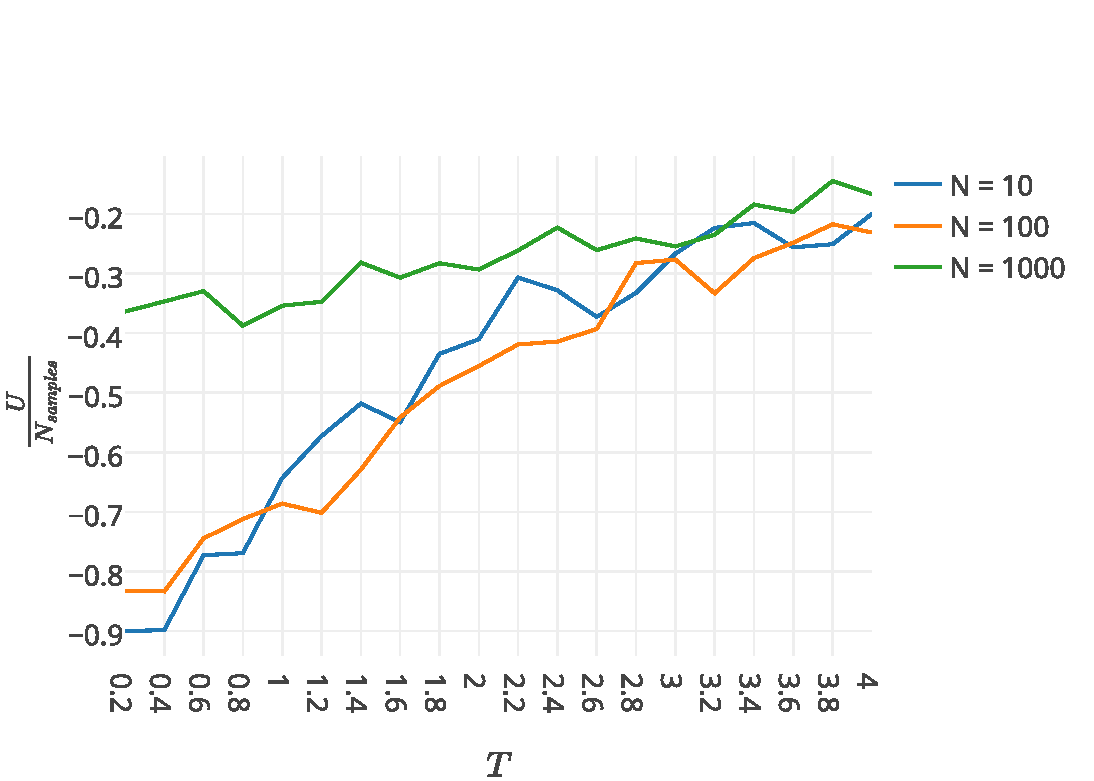
\includegraphics[width=\textwidth, keepaspectratio=true]{img/1D/1DaverageEnergyN1000.pdf}
			\caption{$\numberOfIterations = 1000$}
			\label{fig:results:1D:U:1000}
		\end{subfigure}
		\begin{subfigure}{0.49\textwidth}
			\centering
			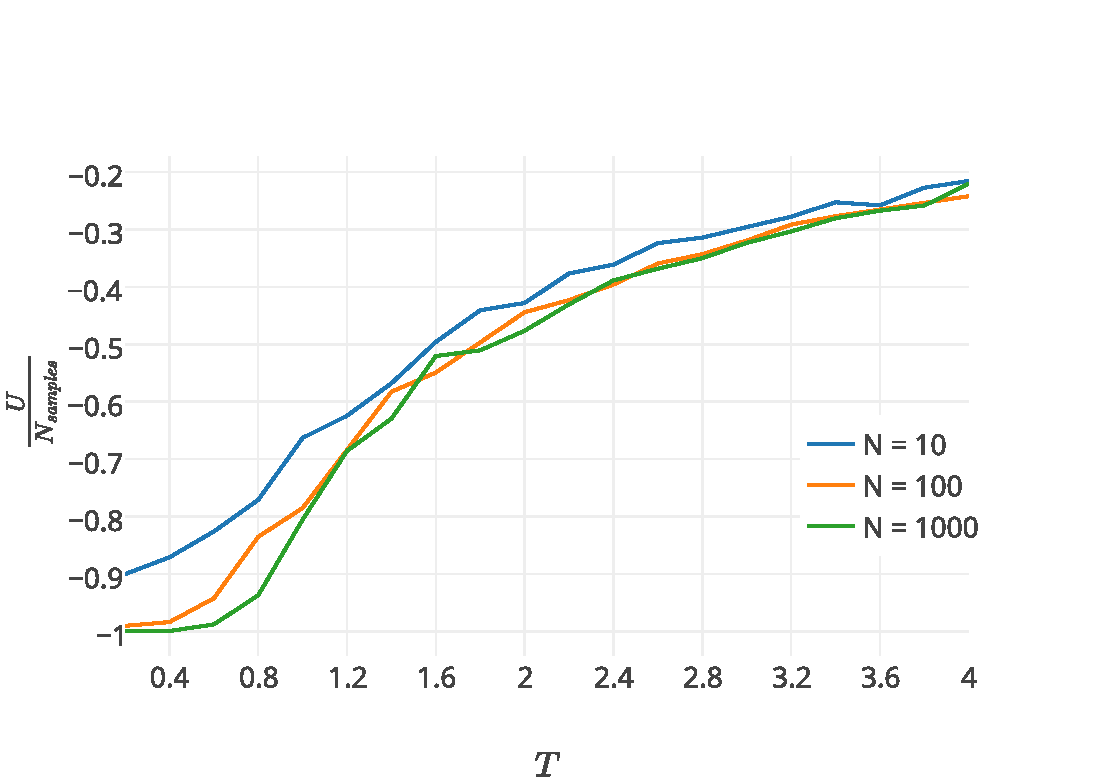
\includegraphics[width=\textwidth, keepaspectratio=true]{img/1D/1DaverageEnergyN10000.pdf}
			\caption{$\numberOfIterations = 10000$}
			\label{fig:results:1D:U:10000}
		\end{subfigure}	
		\caption{The average energy $\averageEnergy$ per spin with \subref{fig:results:1D:U:1000} 1000 and \subref{fig:results:1D:U:10000} 10000 sample iterations, for $T = 0.2, 0.4, \dotsc, 4$ and $\numberOfSpins$, the number of spins, is either 10, 100 or 1000.}
		\label{fig:results:1D:U}
	\end{figure}

	\begin{figure}
		\centering
		\begin{subfigure}{0.49\textwidth}
			\centering
			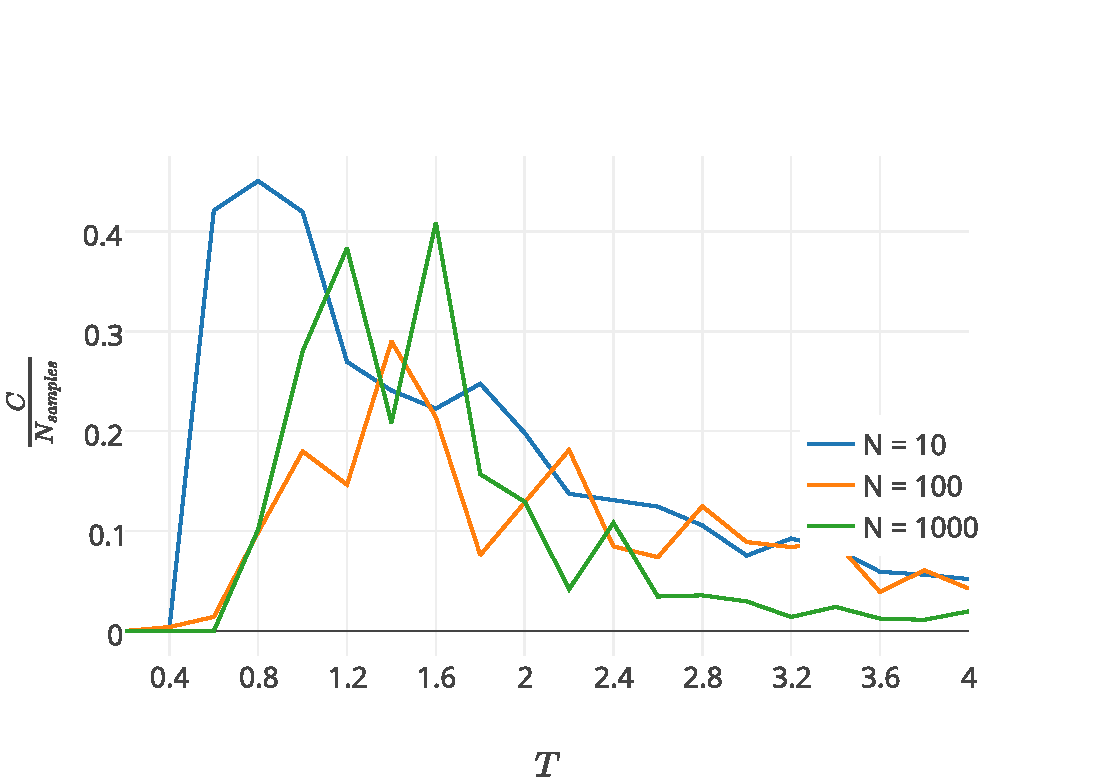
\includegraphics[width=\textwidth, keepaspectratio=true]{img/1D/1DspecificHeatN1000.pdf}
			\caption{$\numberOfIterations = 1000$}
			\label{fig:results:1D:C:1000}
		\end{subfigure}
		\begin{subfigure}{0.49\textwidth}
			\centering
			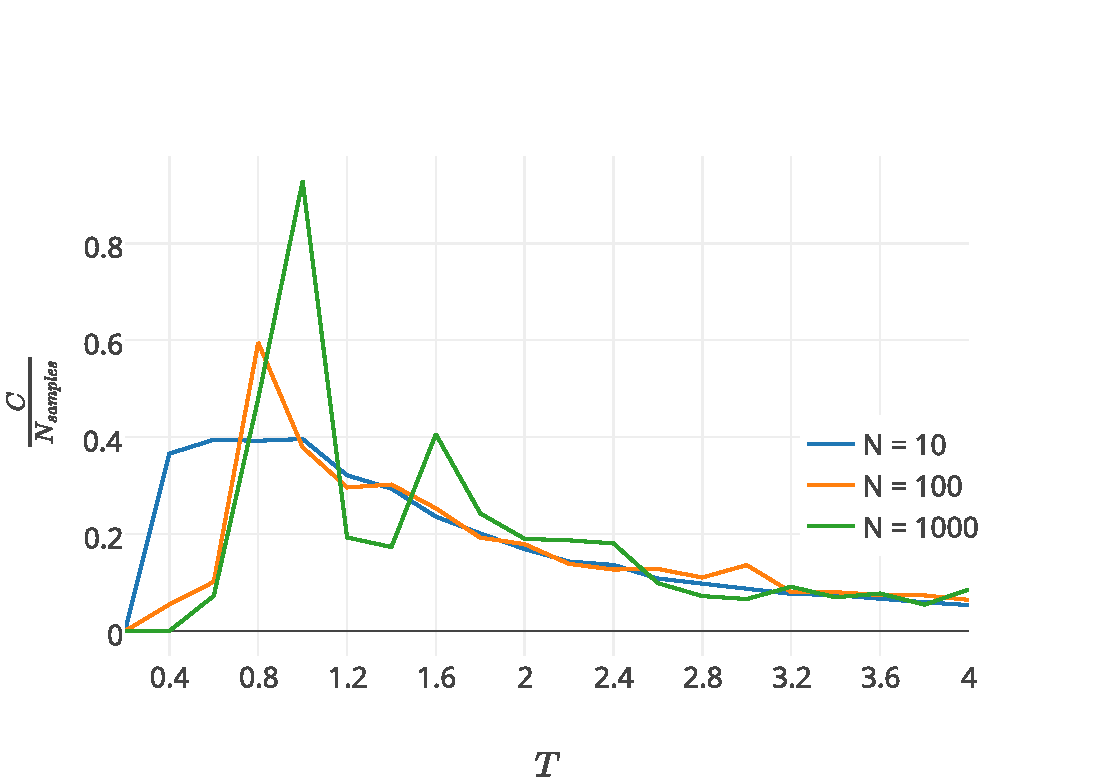
\includegraphics[width=\textwidth, keepaspectratio=true]{img/1D/1DspecificHeatN10000.pdf}
			\caption{$\numberOfIterations = 10000$}
			\label{fig:results:1D:C:10000}
		\end{subfigure}	
		\caption{The specific heat $\specificHeat$ per spin with \subref{fig:results:1D:C:1000} 1000 and \subref{fig:results:1D:C:10000} 10000 sample iterations, for $T = 0.2, 0.4, \dotsc, 4$ and $\numberOfSpins$, the number of spins, is either 10, 100 or 1000.}
		\label{fig:results:1D:C}
	\end{figure}

\subsection{Two-Dimensional Model}
	\todo[inline]{Wat gaan we doen?}

	\subsubsection*{Average Energy}
		\todo[inline]{Report average energy for different values of T, N and NSAMPLES}


	\subsubsection*{Specific Heat}
		\todo[inline]{Report specific heat for different values of T, N and NSAMPLES}

	\subsubsection*{Average Magnetization}
		\todo[inline]{Report average magnetization for different values of T, N and NSAMPLES}	